\documentclass{article}

\usepackage{enumitem}
\usepackage{listings}
\usepackage{color}
\usepackage{amsmath}
\usepackage{hyperref}
\usepackage{graphicx}
\usepackage{pgffor}
\usepackage{xparse}
\usepackage{expl3}
\usepackage{tabularx, makecell}
\usepackage{booktabs}
\usepackage{indentfirst}
\usepackage{lipsum}
\usepackage{sectsty}
\usepackage[utf8]{inputenc}
\usepackage{csquotes}
\usepackage{xcolor}
\usepackage{fancyvrb}
\usepackage{fancyhdr}
\usepackage{fancyvrb}
\usepackage[most]{tcolorbox}
\usepackage{blindtext}
\usepackage{caption}
\usepackage{etoolbox}
\usepackage{booktabs}
\usepackage{karnaugh-map}
\usepackage{tikz}
\usepackage{mdframed}

\graphicspath{{./}}

\definecolor{codegreen}{rgb}{0,0.6,0}
\definecolor{codegray}{rgb}{0.5,0.5,0.5}
\definecolor{codepurple}{rgb}{0.58,0,0.82}
\definecolor{backcolour}{rgb}{0.95,0.95,0.92}

\sectionfont{\bfseries\Large\center} 

% Lstlisting configuartions for C++
\lstset{
	language=C++,
	frame=single,
	rulecolor=\color{gray},
	basicstyle=\fontsize{5}{5}\ttfamily,
	keywordstyle=\color{blue},
	stringstyle=\color{orange},
	commentstyle=\color{gray},
	extendedchars=true,
	keepspaces=true,
	numbers=left,
	numbersep=5pt,
	numberstyle=\color{gray},
	tabsize=4,
	morecomment=[l][\color{gray}]{\#}
}

% Lstlisting configuartions for algorithm code
\newcounter{nalg}[section]
\renewcommand{\thenalg}{\arabic{nalg}}
\DeclareCaptionLabelFormat{algocaption}{\textbf{Algorithm \thenalg}}
\lstnewenvironment{algorithm}[1][]
{
    \refstepcounter{nalg}
    \captionsetup{labelformat=algocaption,labelsep=colon}
    \lstset{
        mathescape=true,
        frame=tB,
        numbers=left, 
        numberstyle=\tiny,
        basicstyle=\scriptsize, 
        keywordstyle=\color{blue}\bfseries\em,
        keywords={,input, output, return, datatype, function, in, if, else, foreach, while, begin, end, then, }
        numbers=left,
        xleftmargin=.04\textwidth,
        #1
    }
}{}

\begin{document}
	% Custom Commands

	% <Square cases>
	\makeatletter
	\newenvironment{sqcases} {
		\matrix@check\sqcases\env@sqcases
	}{
		\endarray \right.
	}
	\def\env@sqcases {
		\let \@ifnextchar \new@ifnextchar
		\left \lbrack
		\def \arraystretch{1.2}
		\array{@{}l@{\quad}l@{}}
	}
	\makeatother
	% </Square cases>

	% Begin of the document

	\title{ASDN laboratory\_01}
	\author{Terman Emil FAF161}
	\maketitle

	% Write at bottom
	\vspace*{\fill}
	
	\centering
	
\includegraphics{imgs/UTM_logo.png}

	\begin{flushright}
		Prof: S. Munteanu
	\end{flushright}

	\LaTeX
	\pagebreak
	% End of title page

	\raggedright
	{\large \textbf{Subject:}} studierea practică şi cercetarea procesului de sinteză a circuitelor logice combinaţionale.
	
	{\large \textbf{Conditions:}}
	\begin{itemize}
		\item \begin{enumerate}
			\item Se verifică  corectitudinea funcţionării circuitelor integrate ale standului de laborator.

			\item Se asamblează şi se reglează circuitul logic combinaţional, care realizează două funcţii din tema pentru acasă în setul de elemente ŞI-NU (la indicaţia profesorului).

			\item Pentru circuitele asamblate se determină costul şi timpul de reţinere.
		\end{enumerate}

		\item \begin{enumerate}
			\item Din biblioteca de elemente Simulation Gates.clf se selectează elementele NAND cu numărul corespunzător de intrări. Din biblioteca Simulation IO.clf se selectează dispozitivele de intrare-ieşire Binary Probe şi Hex Keyboard.

			\item Se asamblează circuitul logic combinaţional în Fereastra de lucru şi se verifică corectitudinea lui. Se studiază diagrama de timp. Un exemplu al circuitului asamblat este prezentat în fig. 2.1.

			\item Pentru circuitele asamblate se determină costul şi timpul de reţinere.
		\end{enumerate}
	\end{itemize}
	%Page 2

	\newpage
	\section{First function} %-------------------------------------First section
		\begin{center}
			$y_1 = \Sigma(0, 1, 2, 4, 5, 8, 9, 12, 14)$
		\end{center}

		\vspace{\fill}
		\subsection{Karnaugh map} %------------------First subsection-----------
			\rule{\textwidth}{0.4pt}
			\begin{center} \begin{tabular}{ll}
				\begin{karnaugh-map}[4][4][1][$x_1x_2$][\rotatebox{90}{$x_3x_4$}]
					\minterms{0,1,2,3,4,5,6,8,11}
					\autoterms[0]

					\implicant{0}{5}
					\implicantedge{0}{0}{8}{8}
					\implicantedge{3}{3}{11}{11}
					\implicantedge{0}{4}{2}{6}
				\end{karnaugh-map}
				&
				\begin{karnaugh-map}[4][4][1][$x_1x_2$][\rotatebox{90}{$x_3x_4$}]
					\minterms{0,1,2,3,4,5,6,8,11}
					\autoterms[0]

					\implicant{12}{14}
					\implicant{13}{9}
					\implicant{7}{15}
					\implicant{14}{10}
				\end{karnaugh-map}
			\end{tabular} \end{center}
			\rule{\textwidth}{0.4pt}
			\vspace{\fill}

		\newpage
		\subsection{Disjunctiv minimal form} %-------Second subsection----------
			\[
				\textbf{$F_{DM}$} =
				(x_1 \cdot x_2 \cdot \overline{x_4}) +
				(\overline{x_2} \cdot \overline{x_3}) +
				(\overline{x_1} \cdot \overline{x_3}) +
				(\overline{x_1} \cdot \overline{x_2} \cdot \overline{x_4})
			\]
			\[
				= \overline{
					(\overline{x_1 \cdot x_2 \cdot \overline{x_4}})
					\cdot
					(\overline{\overline{x_2} \cdot \overline{x_3}})
					\cdot
					(\overline{\overline{x_1} \cdot \overline{x_3}})
					\cdot
					(\overline{\overline{x_1} \cdot \overline{x_2} \cdot \overline{x_4}})
				}
			\]

			\begin{center} \begin{figure}[!ht]
				\begin{mdframed} \begin{center}
					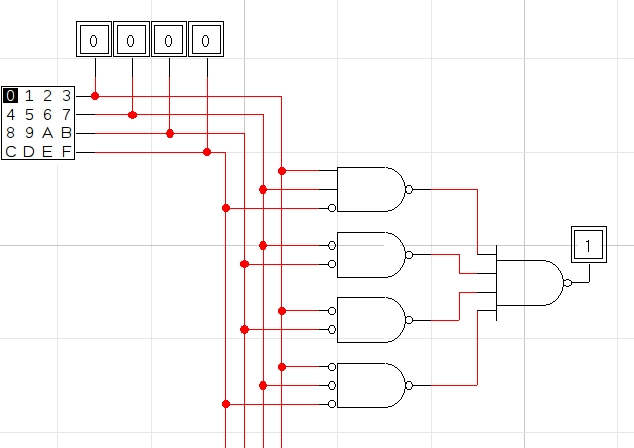
\includegraphics[scale=0.5]{./imgs/Circuit1_FDM_ex1.jpg}
					\caption{Circuit $y_1$, $F_{DM}$.}
				\end{center} \end{mdframed}
				\label{fig:circuit_y1_fdm}
			\end{figure} \end{center}
			
			\begin{center} \begin{figure}[!ht]
				\begin{mdframed} \begin{center}
					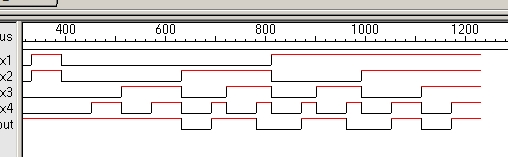
\includegraphics[scale=0.5]{./imgs/Circuit1_FDM_ex1_timer.jpg}
					\caption{Circuit $y_1$, $F_{DM}$ Timer.}
				\end{center} \end{mdframed}
				\label{fig:circuit_y1_fdm_timer}
			\end{figure} \end{center}

			\begin{center}
				\par C = 14Q
				\par $T_d = 2r$
			\end{center}
			\pagebreak

		\newpage
		\subsection{Conjunctive minimal form} %-------Third subsection----------
			\[
				\textbf{$F_{CM}$} = 
				(x_1 + \overline{x_2} + \overline{x_3}) \cdot
				(\overline{x_1} + \overline{x_2} + \overline{x_4}) \cdot
				(\overline{x_1} + x_2 + \overline{x_3}) \cdot
				(\overline{x_3} + \overline{x_4})
			\]
			\[
				= \overline{
					(\overline{x_1 + \overline{x_2} + \overline{x_3}}) +
					(\overline{\overline{x_1} + \overline{x_2} + \overline{x_4}}) +
					(\overline{\overline{x_1} + x_2 + \overline{x_3}}) +
					(\overline{\overline{x_3} + \overline{x_4}})
				}
			\]

			\begin{center} \begin{figure}[!ht]
				\begin{mdframed} \begin{center}
					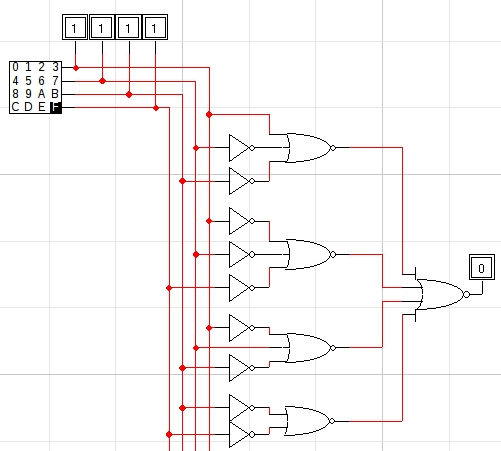
\includegraphics[scale=0.5]{./imgs/Circuit1_FCM_ex1.jpg}
					\caption{Circuit $y_1$, $F_{CM}$.}
				\end{center} \end{mdframed}
				\label{fig:circuit_y1_fcm}
			\end{figure} \end{center}
		
			\begin{center} \begin{figure}[!ht]
				\begin{mdframed} \begin{center}
					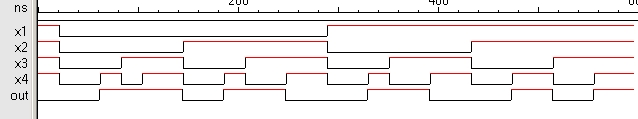
\includegraphics[scale=0.4]{./imgs/Circuit1_FCM_ex1_timer.jpg}
					\caption{Circuit $y_1$, $F_{CM}$ Timer.}
				\end{center} \end{mdframed}
				\label{fig:circuit_y1_fcm_timer}
			\end{figure} \end{center}

			\begin{center}
				\par C = 24Q
				\par $T_d = 3r$
			\end{center}
			\pagebreak

	\newpage
	\section{Second function} %-----------------------------------Second section
		\begin{center}
			$y_1 = \Sigma(1, 2, 3, 5, 6, 8, 10, 11, 12)$
		\end{center}

		\vspace{\fill}
		\subsection{Karnaugh map} %-------------------First subsection----------
			\rule{\textwidth}{0.4pt}
			\begin{center}\begin{tabular}{ll}
				\begin{karnaugh-map}[4][4][1][$x_1x_2$][\rotatebox{90}{$x_3x_4$}]
					\minterms{2,3,4,5,8,9,10,12,14}
					\autoterms[0]

					\implicant{3}{2}
					\implicant{4}{5}
					\implicant{8}{9}
					\implicantedge{12}{8}{14}{10}
				\end{karnaugh-map}
				&
				\begin{karnaugh-map}[4][4][1][$x_1x_2$][\rotatebox{90}{$x_3x_4$}]
					\minterms{2,3,4,5,8,9,10,12,14}
					\autoterms[0]

					\implicant{0}{1}
					\implicant{7}{6}
					\implicant{13}{15}
					\implicant{15}{11}
				\end{karnaugh-map}
			\end{tabular}\end{center}
			\rule{\textwidth}{0.4pt}
			\vspace{\fill}

		\newpage
		\subsection{Disjunctiv minimal form} %-------Second subsection----------
			\[
				\textbf{$F_{DM}$} =
					x_1 \cdot \overline{x_3} \cdot \overline{x_4} +
					\overline{x_1} \cdot \overline{x_3} \cdot x_4 +
					\overline{x_1} \cdot x_3 \cdot \overline{x_4} +
					\overline{x_2} \cdot x_3
			\]
			\[
				= \overline{
					(\overline{x_1 \cdot \overline{x_3} \cdot \overline{x_4}}) \cdot
					(\overline{\overline{x_1} \cdot \overline{x_3} \cdot x_4}) \cdot
					(\overline{\overline{x_1} \cdot x_3 \cdot \overline{x_4}}) \cdot
					(\overline{\overline{x_2} \cdot x_3})
				}
			\]

			\begin{center} \begin{figure}[!ht]
				\begin{mdframed} \begin{center}
					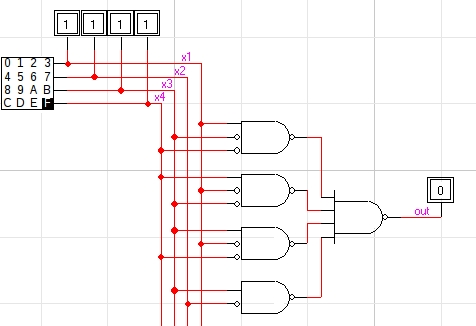
\includegraphics[scale=0.5]{./imgs/Circuit1_FDM_ex2.jpg}
					\caption{Circuit $y_2$, $F_{DM}$.}
				\end{center} \end{mdframed}
				\label{fig:circuit_y2_fdm}
			\end{figure} \end{center}
			
			\begin{center} \begin{figure}[!ht]
				\begin{mdframed} \begin{center}
					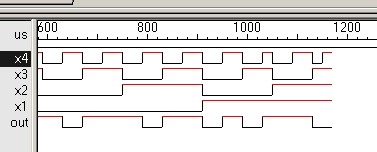
\includegraphics[scale=0.5]{./imgs/Circuit1_FDM_ex2_timer.jpg}
					\caption{Circuit $y_2$, $F_{DM}$ Timer.}
				\end{center} \end{mdframed}
				\label{fig:circuit_y2_fdm_timer}
			\end{figure} \end{center}

			\begin{center}
				\par C = 15Q
				\par $T_d = 2r$
			\end{center}
			\pagebreak

		\newpage
		\subsection{Conjunctiv minimal form} %--------Third subsection----------
			\[
				\textbf{$F_{CM}$} =
					(x_1 + x_3 + x_4) \cdot
					(\overline{x_1} + x_3 + \overline{x_4}) \cdot
					(\overline{x_2} + \overline{x_3} + \overline{x_4}) \cdot
					(\overline{x_1} + \overline{x_2} + \overline{x_3})
			\]
			\[
				= \overline{
					(\overline{x_1 + x_3 + x_4}) +
					(\overline{\overline{x_1} + x_3 + \overline{x_4}}) +
					(\overline{\overline{x_2} + \overline{x_3} + \overline{x_4}}) +
					(\overline{\overline{x_1} + \overline{x_2} + \overline{x_3}})
				}
			\]

			\begin{center} \begin{figure}[!ht]
				\begin{mdframed} \begin{center}
					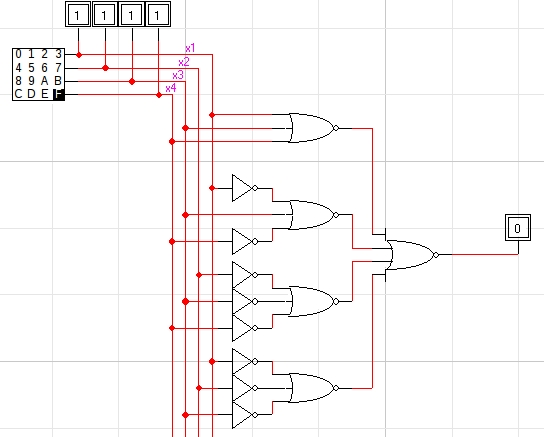
\includegraphics[scale=0.5]{./imgs/Circuit1_FCM_ex2.jpg}
					\caption{Circuit $y_2$, $F_{CM}$.}
				\end{center} \end{mdframed}
				\label{fig:circuit_y2_fcm}
			\end{figure} \end{center}
		
			\begin{center} \begin{figure}[!ht]
				\begin{mdframed} \begin{center}
					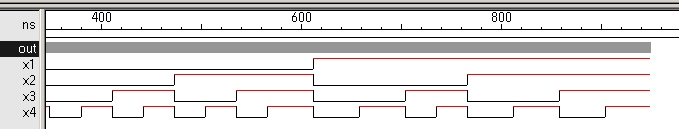
\includegraphics[scale=0.4]{./imgs/Circuit1_FCM_ex2_timer.jpg}
					\caption{Circuit $y_2$, $F_{CM}$ Timer.}
				\end{center} \end{mdframed}
				\label{fig:circuit_y2_fcm_timer}
			\end{figure} \end{center}

			\begin{center}
				\par C = 24Q
				\par $T_d = 3r$
			\end{center}
			\pagebreak

	\newpage
	\section{Conclusion} %-----------------------------------------Third section
		\begin{itemize}
			\item De Morgan's laws help us very much in minimizing the expression. It allows us to use only one type of gate. In this way, we can create a much cheaper circuit, since we have to buy only one kind of gate.

			\item Karnaugh maps are a much better representation of a circuit than a truth table. But we can't represent the circuits with too many signals in it.
		\end{itemize}

\end{document}
